%****************************************************
\begin{frame}{\bf Pautas da reunião}
\begin{itemize}
\justifying
\item \textbf{Geral}: Atualização do PPC da ECA
\item \textit{\textbf{Específicos}}:
\begin{itemize}
	\justifying
	\item Criação da comissão de alteração/atualização do PPC do curso de ECA;
	\item Formalização do avanço dos trabalhos de alteração do PPC no SEI;
	\item Discussões basilares sobre números do curso de ECA;
	\item Plano de ações e metodologia de trabalho;
	\item Pauta correlata.
\end{itemize}


\end{itemize}

\end{frame}
%****************************************************
\begin{frame}{\bf O que deve ser entregue?}

Atualização do PPC da ECA em conformidade com:\\

\begin{enumerate}
\justifying
\item Resolução n.º 02 do CNE/CES: Diretrizes Curriculares Nacionais(DCNs) para Engenharia.
\vspace{0.5cm}
\item Resolução n.º 259 do CONSUP: Manual de Normalização de Projetos
Pedagógicos dos Cursos de Engenharia do IFCE;
\vspace{0.5cm}
\item Guia da curricularizacao da extensão IFCE;
\vspace{0.5cm}
\item Instrumento de avaliação de cursos de graduação.

\end{enumerate}

\end{frame}
%****************************************************
\begin{frame}{\bf Quando deve ser entregue?}
	
Primeira data era 24 de março de 2019, com prazo de 3 anos para adequação.\\
\textbf{Segunda data:} 24 de março de 2027.\\

\textbf{Fluxo:}	
	\begin{enumerate} \small
		\justifying
		\item NDE
		\item Colegiado da ECA
		\item CTP
		\item Núcleos de Apoio: (NAPNE, NEABI, NUGEDS, NTEaD)
		\item Setor de Extensão
		\item DE
		\item DG
		\item PROEN
		\item CONSUP
	\end{enumerate}
	30 dias em cada área = 8 meses $\rightarrow$ Saída do NDE em: ?
\end{frame}

%****************************************************
\begin{frame}{\bf Quando deve ser entregue? Marco}
	
	\textbf{Fluxo:}	
	\begin{enumerate} \small
		\justifying
		\item 2025: 3 meses ( Out, Nov, Dez )
		\item 2026: 10 meses (Fev, Mar, Abr, Maio, Jun, Ago, Set, Out, Nov, Dez)
		\item 2027: 2 meses (Fev, Mar)
	\end{enumerate}
	Disponível : 15 meses\\
	Fluxo: 8 meses\\
	Tempo de alteração na ECA: 7 meses\\
	
	Saída do NDE em: \textcolor{red}{\textbf{Maio/2026}}
\end{frame}

%****************************************************
\begin{frame}{\bf Metodologia}
\begin{minipage}{9.5cm}
	\begin{figure}
	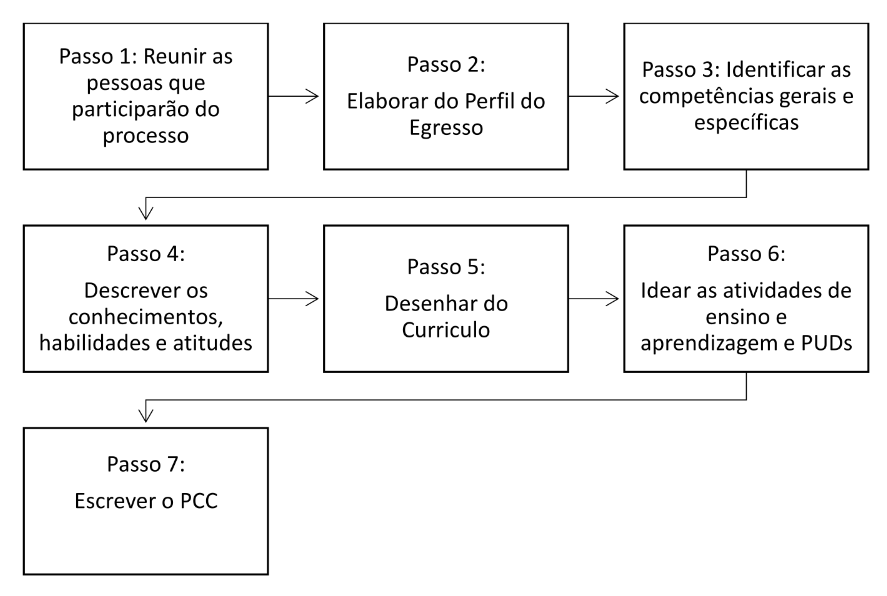
\includegraphics[scale=0.3]{figures/Fluxo_proposto}
	\vspace{-.15cm}
    \caption*{Fonte: Manual de atualização de PPC Engenharia IFCE }
	\end{figure}
\end{minipage}
\begin{minipage}{6cm}	
	Ocasião para:
	
	\begin{itemize}
		\item Rever \textit{design} do curso
		\item Ajustar PPC
		\item Incluir disciplinas
		\item Excluir disciplinas
		\item Converter ações em curriculo
		\item Incluir disciplinas à noite
	\end{itemize}
	\vfill
\end{minipage}	
	
\end{frame}

%****************************************************

\begin{frame}{Visão geral}
	\centering
	\vspace{-.2cm}
	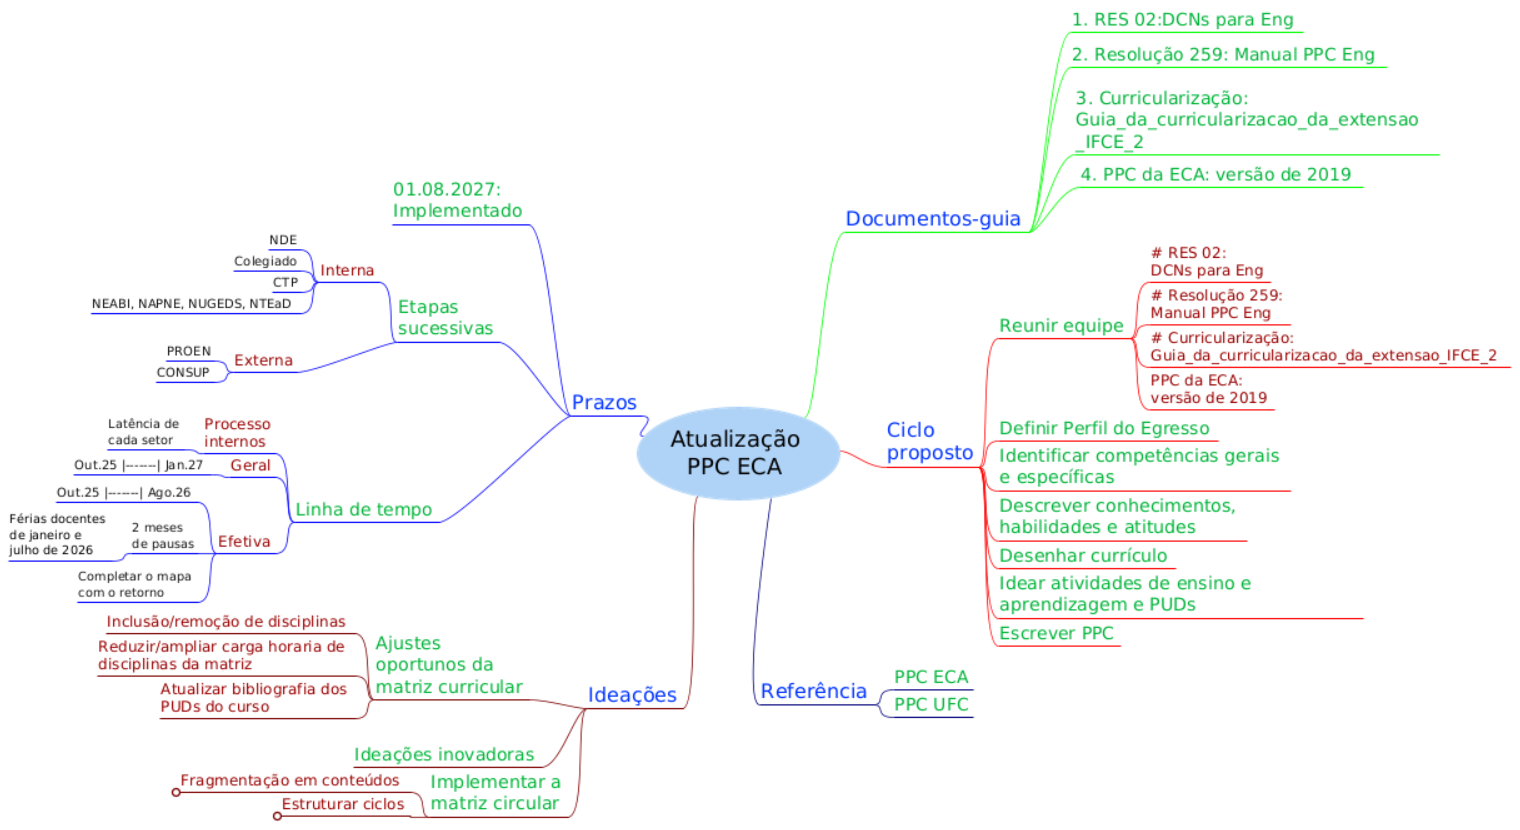
\includegraphics[scale=0.275]{figures/MapaECA_Atual}
\end{frame}
%****************************************************

\begin{frame}{Plano de Ação - Curso de Engenharia de Controle e Automação}
	\centering \scriptsize 
	\renewcommand{\arraystretch}{1.5} % espaçamento entre linhas
	\setlength{\tabcolsep}{6pt}       % espaçamento entre colunas
	\begin{tabular}{p{3.5cm} p{2.5cm} p{4cm} p{3cm}} 
		\toprule
		\textbf{O que} & \textbf{Quando} & \textbf{Como} & \textbf{Quem} \\
		\midrule
		
		Estudo dos documentos-guia & \textcolor{blue}{Outubro/2025} & Análise coletiva do NDE e docentes do curso & NDE e Coordenação do Curso \\
		
		Atualização das ementas e PUDs & \textcolor{blue}{Novembro/2025} & Reuniões com docentes e validação em colegiado & Docentes responsáveis por disciplinas \\
		
		Ajustes do documento PPC& \textcolor{blue}{Dezembro/2025} & Documento em latex & Coordenação de Curso \\
		
		Minuta & \textcolor{blue}{Fevereiro/2026} & Reunião geral e comunicação aos alunos & Coordenação e Secretaria Acadêmica \\
		
				
		 - & \textcolor{blue}{-} & - & - \\
		\bottomrule
		\bottomrule
	\end{tabular}
\end{frame}

%****************************************************

\begin{frame}{Situação das Matrículas}
	\centering
	\renewcommand{\arraystretch}{1.3}
	\setlength{\tabcolsep}{10pt}
	
	\begin{table}[h!]
		\centering
		\caption{Situação geral dos discentes da ECA: 2025.2}
		\begin{tabular}{l|c}
			\hline
			\textbf{Desc\_Sit\_Matricula} & \textbf{Contagem de Matrícula} \\
			\hline
			Abandono & 131 \\
			Cancelado Compulsoriamente & 21 \\
			Cancelado Voluntariamente & 49 \\
			Formado & 28 \\
			Matriculado & 161 \\
			Trancado & 5 \\
			Transferido Externo & 31 \\
			Transferido Interno & 9 \\
			\hline
			\textbf{Resultado} & \textbf{435} \\
			\hline
		\end{tabular}
		\caption*{Fonte: Q-Acadêmico. 2025.2}
	\end{table}
\end{frame}

\begin{frame}{Ingresso por Ano Letivo}
	\centering
	\renewcommand{\arraystretch}{1.3}
	\setlength{\tabcolsep}{10pt}
	\scriptsize 
	\begin{table}[h!]
		\centering
		\caption{\small Matrículas em 10 anos}
		\begin{tabular}{c|c}
			\hline
			\textbf{ano\_letivo\_ini} & \textbf{Contagem de Matrícula} \\
			\hline
			2015 & 5 \\
			2016 & 7 \\
			2017 & 5 \\
			2018 & 11 \\
			2019 & 15 \\
			2020 & 8 \\
			2021 & 14 \\
			2022 & 21 \\
			2023 & 16 \\
			2024 & 29 \\
			2025 & 30 \\
			\hline
			\textbf{Resultado} & \textbf{161} \\
			\hline
		\end{tabular}
	\end{table}
\end{frame}



\begin{frame}{Material disponível}
\begin{itemize}
	\item Material geral disponível em: \url{https://classroom.google.com/c/ODA4NjU5MDc1OTAy?cjc=cymdj5ep}
\end{itemize}

\end{frame}

